\input{../../Plantillas-Fomato/Tareas/tarea.tex}
\cabe{Geometría \textsc{iii}: Tarea 2}{Jhonny Lanzuisi, 1510759}

\begin{document}
		\thispagestyle{plain}
		\tituloD{Geometría 3}{Segunda Tarea}
		\subsection*{Ejercicio 1}
		Sean $c'$ y $c$ dos circunferencias tangentes exteriores. Sea $t$ una de las tengentes exteriores a $c$ y $c'$ sean $A$ y $B$ los puntos de tangencia de $t$ con las circunferencias $c$ y $c'$. Demuestre que la circunferencia de diámetro $AB$ pasa por $P$ (donde $P$ es el punto de tangencia entre $c$ y $c'$) y es tangente a la recta $OO'$.
		
		\begin{sol}
			La perpendicular por $P$ a la recta $OO'$ corta al segmento $AB$ en un punto $O''$. Los triángulos $\triangle O''PO'$ y $\triangle O''BO'$ son congruentes puesto que comparten hipotenusa y $O'P=O'B$. Por un razonamiento análogo los triangulos $OAO''$ y $OPO''$ son congruentes. Como $AO''=BO''=PO''$ que es el radio, se obtiene el resultado deseado.
			\begin{figure}[H]\centering
				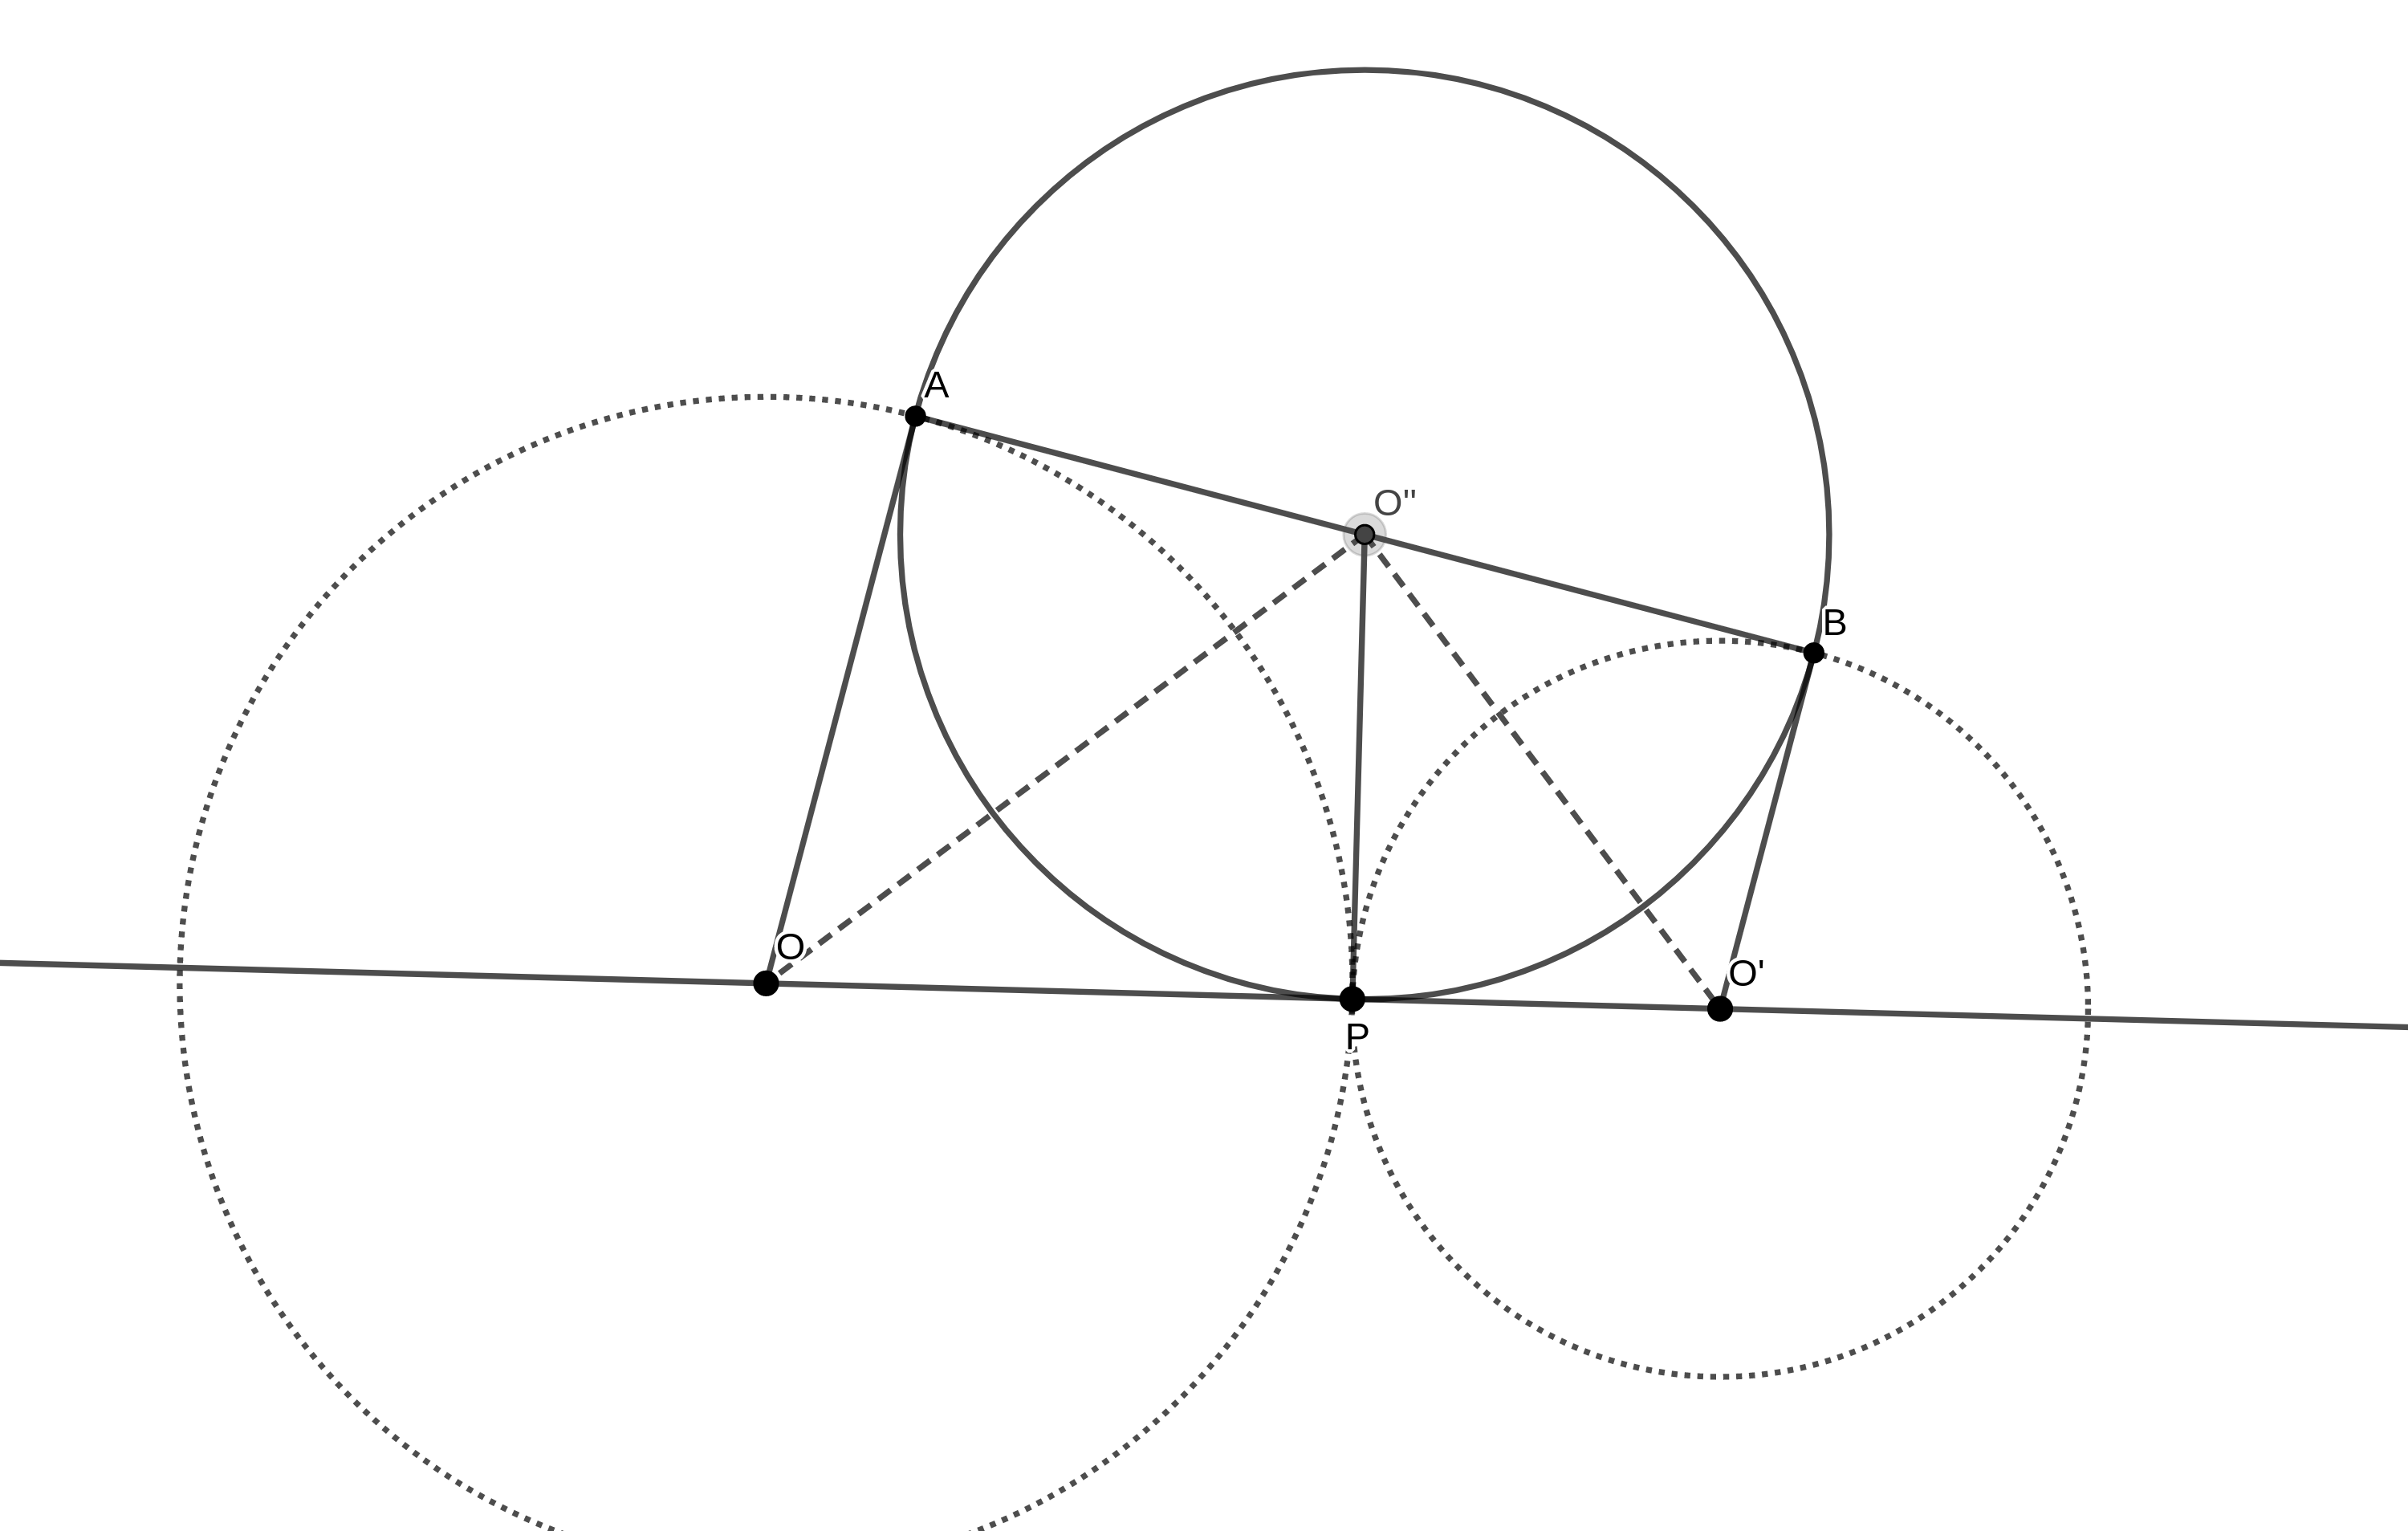
\includegraphics[width=1\linewidth]{pics/g3}
			\end{figure}
		\end{sol}
\end{document}